\documentclass[aspectratio=169, handout]{beamer}

%\usepackage[table]{xcolor}
\mode<presentation> {
\setbeamercovered{transparent}
  \usetheme{Boadilla}

\renewcommand{\familydefault}{cmss}
\usepackage{bm}
\usepackage{listings}
\useinnertheme{rectangles}
}
\usepackage{amsmath}
\usepackage{bbold}
\usepackage{tcolorbox}
\setbeamercolor{normal text}{fg=black}
\setbeamercolor{structure}{fg= blue}
\definecolor{trial}{cmyk}{1,0,0, 0}
\definecolor{trial2}{cmyk}{0.00,0,1, 0}
\definecolor{darkgreen}{rgb}{0,.4, 0.1}
\definecolor{darkpurple}{rgb}{0.4, 0, 0.6}
\usepackage{array}
\beamertemplatesolidbackgroundcolor{white}  \setbeamercolor{alerted
text}{fg=darkpurple}
\setbeamertemplate{caption}[numbered]\newcounter{mylastframe}

\font\domino=domino
\def\die#1{{\domino#1}}
\usepackage{tikz}
\usetikzlibrary{arrows}
\usepackage{colortbl}

\renewcommand{\familydefault}{cmss}

\usepackage{tikz}
\usepackage{lipsum}
\usepackage{booktabs}

\lstset{%
  language=R,
  basicstyle=\ttfamily\small,
  keywordstyle=\color{blue},
  commentstyle=\color{darkgreen},
  stringstyle=\color{darkpurple},
  showstringspaces=false,
  breaklines=true,
  frame=single,
  backgroundcolor=\color{gray!10}
}

 \newenvironment{changemargin}[3]{%
 \begin{list}{}{%
 \setlength{\topsep}{0pt}%
 \setlength{\leftmargin}{#1}%
 \setlength{\rightmargin}{#2}%
 \setlength{\topmargin}{#3}%
 \setlength{\listparindent}{\parindent}%
 \setlength{\itemindent}{\parindent}%
 \setlength{\parsep}{\parskip}%
 }%
\item[]}{\end{list}}
\usetikzlibrary{arrows}
\usetikzlibrary{arrows.meta, positioning}
\usepackage{pgfplots}
\pgfplotsset{compat=1.17}
\usecolortheme{lily}

\newtheorem{com}{Comment}
\newtheorem{lem} {Lemma}
\newtheorem{prop}{Proposition}
\newtheorem{condition}{Condition}
\newtheorem{thm}{Theorem}
\newtheorem{defn}{Definition}
\newtheorem{cor}{Corollary}
\newtheorem{obs}{Observation}
 \numberwithin{equation}{section}

\makeatletter
\def\beamerorig@set@color{%
  \pdfliteral{\current@color}%
  \aftergroup\reset@color
}
\def\beamerorig@reset@color{\pdfliteral{\current@color}}
\makeatother
\setbeamertemplate{navigation symbols}{}

\useoutertheme{miniframes}
\title[PLSC 30700]{Linear Models Lecture 14: 2SLS, LATE, and the MTE Framework}

\author{Robert Gulotty}
\institute[Chicago]{University of Chicago}
\vspace{0.3in}


\begin{document}

\begin{frame}
\maketitle
\end{frame}

%%%%%%%%%%%%%%%%%%%%%%%%%%%%%%%%%%%%%%%%%%%%%%%%%%%
\section{Control Function}
%%%%%%%%%%%%%%%%%%%%%%%%%%%%%%%%%%%%%%%%%%%%%%%%%%%

\begin{frame}{Control Function Regression}
\begin{itemize}
\item Structural model with endogenous $X_2$:
$$Y=\bm{x}_1'\beta_1+\bm{x}_2'\beta_2+e$$
$$\bm{x}_2=\Gamma'_{12}\bm{z}_1+\Gamma'_{22}\bm{z}_2+u_2$$
\item The \textbf{control function} approach directly models the dependence between $e$ and $u_2$:
$$e=u_2'\alpha+v, \qquad \alpha=(E[u_2u_2'])^{-1}E[u_2e], \qquad E[u_2v]=0$$
\item Substituting into the structural equation:
$$Y=X_1'\beta_1+X_2'\beta_2+u_2'\alpha+v$$
\item After controlling for $u_2$: $E[X_1v]=E[X_2v]=E[u_2v]=0$.
\end{itemize}
\end{frame}


\begin{frame}{Control Function: Implementation}
\begin{itemize}
\item \textbf{Step 1:} Estimate the first stage by OLS to get residuals:
$$\hat{u}_{2i}=X_{2i}-\hat{\Gamma}'_{12}Z_{1i}-\hat{\Gamma}'_{22}Z_{2i}$$
\item \textbf{Step 2:} Include $\hat{u}_2$ as an additional regressor:
$$Y=X\hat{\beta}+\hat{U}_2\hat{\alpha}+\hat{v}$$
\item This is ``subtracting off the endogenous part'' of $X_2$.
\item Under homoskedasticity, the control function estimator of $\beta$ is numerically identical to 2SLS.
\item The coefficient $\hat{\alpha}$ directly tests endogeneity --- if $\alpha=0$, then $X_2$ is exogenous.
\end{itemize}
\end{frame}


\begin{frame}[fragile]{R: Control Function}
\begin{lstlisting}
# Step 1: First stage
first_stage <- lm(X2 ~ Z1 + Z2, data = dat)
dat$u2_hat <- residuals(first_stage)

# Step 2: Structural equation with control
cf_reg <- lm(Y ~ X1 + X2 + u2_hat, data = dat)
summary(cf_reg)
# coef on u2_hat tests endogeneity (t-test on alpha)
# coef on X2 is the IV estimate of beta_2
\end{lstlisting}
\begin{tcolorbox}[colback=blue!5, colframe=blue!50]
The control function makes identification transparent: we ``control for'' the endogenous component of $X_2$.  The $t$-test on $\hat{\alpha}$ is equivalent to the Hausman test.
\end{tcolorbox}
\end{frame}


%%%%%%%%%%%%%%%%%%%%%%%%%%%%%%%%%%%%%%%%%%%%%%%%%%%
\section{Finite Sample Properties}
%%%%%%%%%%%%%%%%%%%%%%%%%%%%%%%%%%%%%%%%%%%%%%%%%%%

\begin{frame}{IV Has No Finite Moments}
\begin{itemize}
\item A striking result (Kinal 1980, Kiviet): the IV estimator has at most $q=l-k$ moments, where $q$ is the number of overidentifying restrictions.
\item When just identified ($q=0$): IV has \alert{no expectation} and \alert{no variance}.
\item Why?  Consider $\hat{\beta}_{IV}=(Z'X)^{-1}Z'Y$.  The denominator $Z'X$ can be arbitrarily close to zero, creating Cauchy-like tails.
\item Consequences:
\begin{itemize}
\item The \textbf{bootstrap fails} in the just-identified case --- it requires finite variance.
\item ``Bias'' is not well-defined in the usual sense --- we work with approximate bias instead.
\end{itemize}
\end{itemize}
\end{frame}


\begin{frame}{Imprecision of IV}
\begin{itemize}
\item Suppose $Z$ and $X$ are scalar, mean zero. Compare asymptotic variances:
\begin{align*}
Avar(\hat{\beta}_{OLS})&=\frac{\sigma_e^2}{n}\cdot\frac{1}{\text{var}(x)}\\[6pt]
Avar(\hat{\beta}_{IV})&=\frac{\sigma_e^2}{n}\cdot\frac{1}{\text{var}(x)}\cdot\frac{1}{\rho^2_{xz}}
\end{align*}
\item Therefore:
$$\boxed{Avar(\hat{\beta}_{IV})=Avar(\hat{\beta}_{OLS})\cdot\frac{1}{\rho^2_{xz}}}$$
\item As $\rho^2_{xz}\rightarrow 0$: $Avar(\hat{\beta}_{IV})\rightarrow \infty$.
\item IV is \textbf{always} less precise than OLS --- the cost of correcting for endogeneity.
\end{itemize}
\end{frame}


%%%%%%%%%%%%%%%%%%%%%%%%%%%%%%%%%%%%%%%%%%%%%%%%%%%
\subsection{Bias Derivation}
%%%%%%%%%%%%%%%%%%%%%%%%%%%%%%%%%%%%%%%%%%%%%%%%%%%

\begin{frame}{Decomposing the IV Estimation Error}
\begin{itemize}
\item Write: $y=X\beta+e$ and $X=Z\pi+v$.  Then:
\end{itemize}
\begin{align*}
\hat{\beta}_{IV}&=(X'P_ZX)^{-1}X'P_Zy\\
&=\beta+(X'P_ZX)^{-1}X'P_Ze\\
&=\beta+(X'P_ZX)^{-1}(\pi'Z'+v')P_Ze\\
&=\beta+\underbrace{(X'P_ZX)^{-1}\pi'Z'e}_{\text{Term A}}+\underbrace{(X'P_ZX)^{-1}v'P_Ze}_{\text{Term B}}
\end{align*}
\begin{itemize}
\item \textbf{Term A:} Involves $Z'e$.  Since $E[Z'e]=0$, this vanishes in expectation.
\item \textbf{Term B:} Involves $v'P_Ze$.  Since $v$ and $e$ are correlated (endogeneity!), this does \textbf{not} vanish.
\item Term B is the source of finite-sample bias.
\end{itemize}
\end{frame}


\begin{frame}{Approximate Bias of IV}
Taking approximate expectations (since exact ones may not exist):
\begin{align*}
E(\hat{\beta}_{IV})-\beta&\approx (E(X'P_ZX))^{-1}E(v'P_Ze)\\
&=(E[(\pi'Z'+v')P_Z(Z\pi+v)])^{-1}E[v'P_Ze]\\
&=(E[\pi'Z'Z\pi]+E[v'P_Zv])^{-1}E[v'P_Ze]
\end{align*}
where the cross terms vanish because $E[Z'v]=0$.

Using $E[v'P_Zv]=\sigma_v^2\cdot p$ and $E[v'P_Ze]=\sigma_{ev}\cdot p$ (where $p=l$ is the number of instruments):
$$E(\hat{\beta}_{IV})-\beta\approx (E[\pi'Z'Z\pi]+\sigma_v^2 p)^{-1}\sigma_{ev}\cdot p$$
\end{frame}


\begin{frame}{Bias in Terms of the F-Statistic}
Dividing numerator and denominator by $\sigma_v^2 p$:
$$E(\hat{\beta}_{IV})-\beta\approx \frac{1}{\left(\dfrac{E[\pi'Z'Z\pi]/p}{\sigma^2_v}+1\right)}\cdot\frac{\sigma_{ev}}{\sigma_v^2}\approx \frac{1}{1+F_{p,n-p}}\cdot\frac{\sigma_{ev}}{\sigma_v^2}$$
\begin{itemize}
\item $F$ is the first-stage F-statistic testing $H_0:\pi=0$.
\item The term $\frac{\sigma_{ev}}{\sigma_v^2}$ is exactly the \textbf{OLS bias} (endogeneity).
\item Key implications:
\begin{itemize}
\item As $F\rightarrow\infty$: bias $\rightarrow 0$ (strong instruments eliminate bias)
\item As $F\rightarrow 0$: bias $\rightarrow \frac{\sigma_{ev}}{\sigma_v^2}$ = OLS bias (IV provides no correction)
\item Adding irrelevant instruments increases $p$, decreases $F$, \alert{increases bias}
\end{itemize}
\end{itemize}
\end{frame}


\begin{frame}{Rule of Thumb and Modern Diagnostics}
\begin{itemize}
\item \textbf{Staiger \& Stock (1997):} Rule of thumb $F>10$ for reliable IV.
\item \textbf{Stock \& Yogo (2005):} Critical values for the F-statistic that ensure IV bias is at most $x\%$ of OLS bias.
\item \textbf{Lee et al.\ (2022):} The $tF$ procedure --- adjust critical values for the $t$-test based on the first-stage $F$.
\item The bias formula explains why:
\begin{itemize}
\item ``Fishing'' for instruments is dangerous --- more instruments $\Rightarrow$ more bias
\item A single strong instrument is often better than many weak ones
\item The just-identified case ($p=k_2$) minimizes the finite-sample bias problem
\end{itemize}
\end{itemize}
\end{frame}


%%%%%%%%%%%%%%%%%%%%%%%%%%%%%%%%%%%%%%%%%%%%%%%%%%%
\section{Weak Instruments}
%%%%%%%%%%%%%%%%%%%%%%%%%%%%%%%%%%%%%%%%%%%%%%%%%%%

\begin{frame}{Weak Instruments: OLS Asymptotic Bias}
Scalar case: single $x$, single instrument $z$.  An instrument is \textbf{weak} if $\rho_{zx}$ is small.
\begin{align*}
\text{plim}\;\hat{\beta}_{OLS}&=\text{plim}\;\frac{\text{cov}(x,y)}{\text{var}(x)}=\text{plim}\;\frac{\text{cov}(x,x\beta+e)}{\text{var}(x)}\\
&=\beta+\text{plim}\;\frac{\text{cov}(x,e)}{\text{var}(x)}\\
&=\beta+\frac{\text{cov}(x,e)}{\sqrt{\text{var}(x)}\sqrt{\text{var}(e)}}\cdot\frac{\sqrt{\text{var}(e)}}{\sqrt{\text{var}(x)}}\\
&=\beta+\rho_{xe}\frac{\sigma_e}{\sigma_x}
\end{align*}
The OLS asymptotic bias is $\rho_{xe}\frac{\sigma_e}{\sigma_x}$.
\end{frame}


\begin{frame}{Weak Instruments: IV Asymptotic Bias}
\begin{align*}
\text{plim}\;\hat{\beta}_{IV}&=\text{plim}\;\frac{\text{cov}(z,y)}{\text{cov}(z,x)}=\beta+\text{plim}\;\frac{\text{cov}(z,e)}{\text{cov}(z,x)}\\[4pt]
&=\beta+\frac{\rho_{ze}}{\rho_{zx}}\cdot\frac{\sigma_e}{\sigma_x}\\[4pt]
&=\beta+\frac{\rho_{ze}}{\rho_{zx}\rho_{xe}}\cdot\underbrace{\rho_{xe}\frac{\sigma_e}{\sigma_x}}_{ABias(\hat{\beta}_{OLS})}
\end{align*}
\begin{itemize}
\item If the instrument is perfectly valid ($\rho_{ze}=0$): IV is consistent regardless of $\rho_{zx}$.
\item If the instrument is even slightly invalid ($\rho_{ze}\neq 0$): weak relevance ($\rho_{zx}\approx 0$) \alert{amplifies} the bias.
\end{itemize}
\end{frame}


\begin{frame}{When IV Is Worse Than OLS}
$$\frac{ABias(\hat{\beta}_{IV})}{ABias(\hat{\beta}_{OLS})}=\frac{\rho_{ze}}{\rho_{zx}\rho_{xe}}$$
If $\frac{\rho_{ze}}{\rho_{zx}\rho_{xe}}\geq 1$, then \alert{IV is more biased than OLS}.
\vspace{0.2cm}
\begin{itemize}
\item \textbf{Example:} $\rho_{xe}=0.5$ (very endogenous $X$), $\rho_{ze}=0.01$ (barely invalid $Z$), $\rho_{zx}=0.019$ (weak instrument):
$$\frac{0.01}{0.019\times 0.5}=1.052 \quad\Rightarrow\quad \text{IV bias exceeds OLS bias}$$
\item Approximate relationship to the F-statistic:
$$\frac{ABias(\hat{\beta}_{IV})}{ABias(\hat{\beta}_{OLS})}\approx \frac{1}{F}$$
An $F$ of 100 means IV is $\sim$1\% as biased as OLS.  An $F$ of 5 means $\sim$20\%.
\end{itemize}
\end{frame}


%%%%%%%%%%%%%%%%%%%%%%%%%%%%%%%%%%%%%%%%%%%%%%%%%%%
\section{Testing}
%%%%%%%%%%%%%%%%%%%%%%%%%%%%%%%%%%%%%%%%%%%%%%%%%%%

\begin{frame}{Testing Endogeneity: Durbin-Wu-Hausman Test}
\begin{itemize}
\item If $X$ is exogenous, both OLS and IV are consistent, but OLS is efficient (BLUE).
\item If $X$ is endogenous, only IV is consistent.
\item The \textbf{Hausman test} compares the two:
$$H=(\hat{\beta}_{IV}-\hat{\beta}_{OLS})'[Avar(\hat{\beta}_{IV})-Avar(\hat{\beta}_{OLS})]^{-1}(\hat{\beta}_{IV}-\hat{\beta}_{OLS})\sim \chi^2_{k_2}$$
\item Rejecting $H_0$: either $X$ is endogenous \textbf{or} $Z$ is an invalid instrument.
\item Equivalent to testing $\hat{\alpha}=0$ in the control function regression.
\end{itemize}
\end{frame}


\begin{frame}{Testing Overidentifying Restrictions: Sargan Test}
\begin{itemize}
\item When $l>k$, we have $q=l-k$ ``extra'' moment conditions.
\item If the model is correct, all moment conditions should be approximately satisfied.
\item The \textbf{Sargan test} (also called Hansen's $J$-test):
$$J = n\cdot\hat{e}'P_Z\hat{e}/\hat{\sigma}^2 \sim \chi^2_q \quad \text{under } H_0$$
where $\hat{e}=Y-X\hat{\beta}_{2SLS}$.
\item Rejecting $H_0$: at least one instrument is invalid (correlated with $e$).
\item \alert{Limitation:} If \textbf{all} instruments are invalid in the same way, the test has no power.
\end{itemize}
\begin{tcolorbox}[colback=blue!5, colframe=blue!50]
\textbf{GMM connection:} The Sargan/$J$-test is the overidentification test of GMM.
\end{tcolorbox}
\end{frame}


\begin{frame}[fragile]{R: IV Estimation and Diagnostics}
\begin{lstlisting}
library(estimatr); library(lmtest)

# 2SLS with robust SEs
iv_fit <- iv_robust(Y ~ X2 + X1 | Z2 + X1, data = dat)
summary(iv_fit)  # coefs, robust SEs, first-stage F

# First-stage F-test (check instrument strength)
first <- lm(X2 ~ Z2 + X1, data = dat)
linearHypothesis(first, "Z2 = 0")

# OLS for comparison
ols_fit <- lm(Y ~ X2 + X1, data = dat)
\end{lstlisting}
\end{frame}


%%%%%%%%%%%%%%%%%%%%%%%%%%%%%%%%%%%%%%%%%%%%%%%%%%%
\section{LATE}
%%%%%%%%%%%%%%%%%%%%%%%%%%%%%%%%%%%%%%%%%%%%%%%%%%%

\begin{frame}{What Does IV Estimate Under Heterogeneity?}
\begin{itemize}
\item So far: IV estimates the ``structural parameter'' $\beta$.
\item But what if treatment effects are \textbf{heterogeneous}?  $\beta_i$ varies across individuals.
\item Angrist \& Imbens (1994): with a binary instrument, IV estimates the \textbf{Local Average Treatment Effect}:
$$\hat{\beta}_{IV} \xrightarrow{p} \text{LATE} = E[Y_i(1)-Y_i(0) \mid \text{Compliers}]$$
\item ``Compliers'' = individuals whose treatment status is changed by the instrument.
\end{itemize}
\end{frame}


\begin{frame}{Compliance Types}
\centering
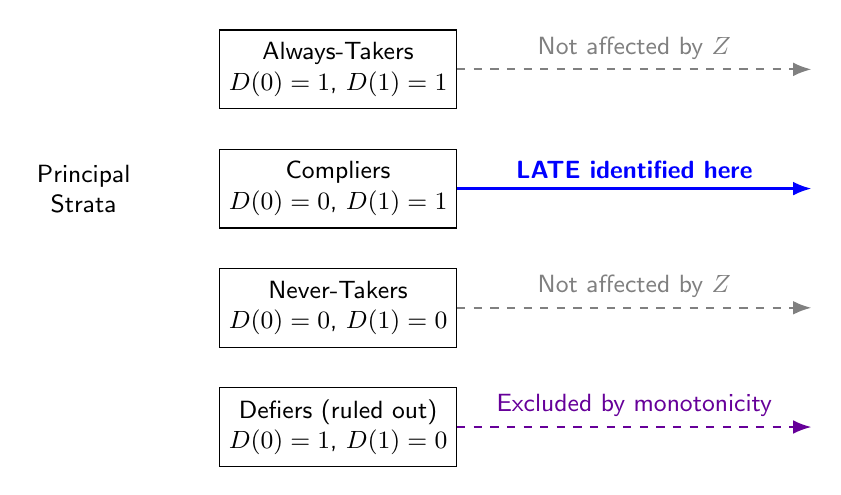
\begin{tikzpicture}[
    node distance=.5cm and 2cm,
    box/.style={rectangle, draw, minimum width=2.8cm, minimum height=1cm, align=center, font=\small},
    arrow/.style={-{Latex}, thick}
]

\node[box] (at) {Always-Takers \\ $D(0) = 1$, $D(1) = 1$};
\node[box, below=of at] (c) {Compliers \\ $D(0) = 0$, $D(1) = 1$};
\node[box, below=of c] (nt) {Never-Takers \\ $D(0) = 0$, $D(1) = 0$};
\node[box, below=of nt] (d) {Defiers (ruled out) \\ $D(0) = 1$, $D(1) = 0$};

\node[left=1cm of c, align=center, font=\small] {Principal\\Strata};

\draw[arrow, blue] (c.east) -- ++(4.5,0) node[midway, above, font=\small] {\textbf{LATE identified here}};
\draw[arrow, dashed, gray] (at.east) -- ++(4.5,0) node[midway, above, font=\small] {Not affected by $Z$};
\draw[arrow, dashed, gray] (nt.east) -- ++(4.5,0) node[midway, above, font=\small] {Not affected by $Z$};
\draw[arrow, darkpurple, dashed] (d.east) -- ++(4.5,0) node[midway, above, font=\small] {Excluded by monotonicity};

\end{tikzpicture}
\end{frame}


\begin{frame}{LATE Assumptions (Angrist-Imbens)}
\begin{tcolorbox}[colback=blue!5, colframe=blue!50]
\textbf{Four assumptions} for LATE identification:
\begin{enumerate}
\item \textbf{Independence:} $(Y_i(0), Y_i(1), D_i(0), D_i(1)) \perp Z_i$
\item \textbf{Exclusion:} $Z_i$ affects $Y_i$ only through $D_i$
\item \textbf{Monotonicity:} $D_i(1) \geq D_i(0)$ for all $i$ (no defiers)
\item \textbf{First stage:} $E[D_i\mid Z_i=1] \neq E[D_i\mid Z_i=0]$
\end{enumerate}
\end{tcolorbox}
\vspace{0.2cm}
Under these assumptions, the Wald estimator identifies:
$$\frac{E[Y_i\mid Z_i=1]-E[Y_i\mid Z_i=0]}{E[D_i\mid Z_i=1]-E[D_i\mid Z_i=0]} = E[Y_i(1)-Y_i(0)\mid \text{Compliers}]$$
LATE is \textbf{instrument-dependent}: different instruments $\Rightarrow$ different compliers $\Rightarrow$ different LATEs.
\end{frame}


\begin{frame}{Example: Returns to Education}
\begin{itemize}
\item Model: $\text{lwage}_i = \alpha + \gamma_1 \text{educ}_i + v_i\cdot\text{educ}_i + u_i$
\item Heterogeneous returns: $\beta_i = \gamma_1 + v_i$
\item If we instrument education with quarter of birth (Angrist \& Krueger 1991):
\begin{itemize}
\item Compliers = those who stay in school because of compulsory schooling laws
\item LATE = return to education for \textbf{marginal students} (those induced to stay)
\item This may differ from ATE or ATT
\end{itemize}
\item \textbf{Policy relevance:} LATE answers ``what is the return for people affected by the policy?'' --- exactly the right parameter for evaluating that policy.
\end{itemize}
\end{frame}


%%%%%%%%%%%%%%%%%%%%%%%%%%%%%%%%%%%%%%%%%%%%%%%%%%%
\section{MTE Framework}
%%%%%%%%%%%%%%%%%%%%%%%%%%%%%%%%%%%%%%%%%%%%%%%%%%%

\begin{frame}{The Generalized Roy Model}
\begin{itemize}
\item Potential outcomes: $Y_i(1)$, $Y_i(0)$ with heterogeneous gains $\Delta_i=Y_i(1)-Y_i(0)$.
\item The treatment decision is based on \textbf{net utility}:
$$D_i^* = \mu_D(Z_i) - U_{Di}$$
$$D_i = \mathbb{1}[D_i^*>0] = \mathbb{1}[\mu_D(Z_i)>U_{Di}]$$
\item $\mu_D(Z_i)$: observable component of the treatment decision (driven by instruments).
\item $U_{Di}$: unobservable \textbf{resistance to treatment} --- the utility cost of participating.
\begin{itemize}
\item Low $U_{Di}$: individual has low cost $\Rightarrow$ eager to participate.
\item High $U_{Di}$: individual has high cost $\Rightarrow$ reluctant to participate.
\end{itemize}
\item Normalize $U_D\sim U[0,1]$ (via probability integral transform).
\end{itemize}
\end{frame}


\begin{frame}{Utility and Selection}
\begin{itemize}
\item In the Roy framework, agents choose treatment when net utility is positive:
$$D_i=1 \quad\Leftrightarrow\quad \underbrace{\text{Expected benefit of treatment}}_{\text{depends on }\Delta_i} > \underbrace{\text{Cost of treatment}}_{U_{Di}}$$
\item The propensity score $P(Z_i)=\Pr(D_i=1\mid Z_i)=\mu_D(Z_i)$ summarizes the instrument.
\item An individual participates iff $U_{Di}\leq P(Z_i)$.
\item \textbf{Key insight:} $U_D$ orders individuals from most to least eager.
\begin{itemize}
\item $U_D\approx 0$: would participate under almost any instrument value (``always-takers'')
\item $U_D\approx 1$: would almost never participate (``never-takers'')
\item $U_D\in[P(z_0), P(z_1)]$: participate when $Z=z_1$ but not $Z=z_0$ (``compliers'')
\end{itemize}
\end{itemize}
\end{frame}


\begin{frame}{The Marginal Treatment Effect (Heckman \& Vytlacil 2005)}
\begin{defn}[Marginal Treatment Effect]
$$\Delta^{MTE}(x, u_D) = E[Y(1)-Y(0)\mid X=x, U_D=u_D]$$
\end{defn}
\begin{itemize}
\item MTE is the treatment effect for individuals \textbf{at the margin} --- those who are just indifferent between treatment and control when their unobserved resistance equals $u_D$.
\item As $u_D$ increases from 0 to 1, we trace out effects from the most eager to the most reluctant:
\begin{itemize}
\item Low $u_D$: low-cost individuals (high utility from treatment) --- often highest returns.
\item High $u_D$: high-cost individuals --- often lowest returns (if gains and costs are correlated).
\end{itemize}
\item MTE is typically \textbf{downward-sloping}: those who self-select into treatment tend to benefit most (essential heterogeneity).
\end{itemize}
\end{frame}


\begin{frame}{All Treatment Parameters as Weighted MTE}
\begin{itemize}
\item Heckman \& Vytlacil's key insight: \textbf{every} treatment parameter is a weighted average of MTE:
$$\Delta^j(x) = \int_0^1 \Delta^{MTE}(x, u_D)\; \omega_j(x, u_D)\; du_D$$
\end{itemize}
\vspace{0.1cm}
\begin{center}
\small
\begin{tabular}{lll}
\toprule
\textbf{Parameter} & \textbf{Weight} $\omega_j$ & \textbf{Who?}\\
\midrule
ATE & 1 & Everyone\\
ATT & $\frac{u_D}{E[D\mid X]}$ (overweights low $u_D$) & Treated\\
ATU & $\frac{1-u_D}{E[1-D\mid X]}$ (overweights high $u_D$) & Untreated\\
LATE & $\frac{1}{u_D'-u_D}\mathbb{1}[u_D\leq t\leq u_D']$ & Compliers\\
\bottomrule
\end{tabular}
\end{center}
\vspace{0.1cm}
\begin{itemize}
\item LATE is MTE averaged over a \textbf{specific interval} of $u_D$ values.
\end{itemize}
\end{frame}


\begin{frame}{Visualizing the MTE Curve}
\begin{center}
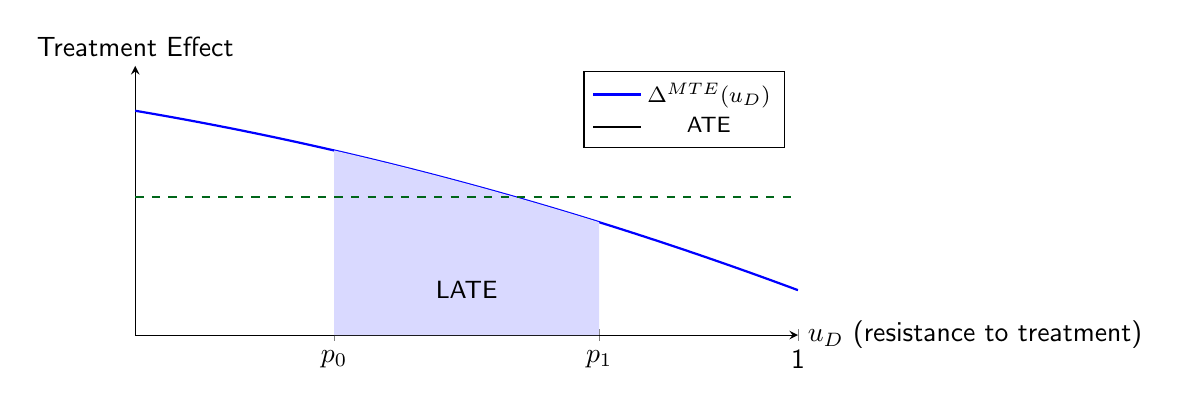
\begin{tikzpicture}
\begin{axis}[
    width=10cm, height=5cm,
    xlabel={$u_D$ (resistance to treatment)},
    ylabel={Treatment Effect},
    xmin=0, xmax=1,
    ymin=0, ymax=1.2,
    axis lines=middle,
    xtick={0, 0.3, 0.7, 1},
    xticklabels={0, $p_0$, $p_1$, 1},
    ytick=\empty,
    every axis x label/.style={at={(ticklabel* cs:1)}, anchor=west},
    every axis y label/.style={at={(ticklabel* cs:1)}, anchor=south},
    legend style={font=\footnotesize, at={(0.98,0.98)}, anchor=north east},
]
\addplot[domain=0:1, samples=100, thick, blue] {1 - 0.5*x - 0.3*x^2};
\addlegendentry{$\Delta^{MTE}(u_D)$}
\addplot[domain=0.3:0.7, samples=50, fill=blue!15, draw=none] {1 - 0.5*x - 0.3*x^2} \closedcycle;
\addplot[domain=0:1, samples=2, dashed, darkgreen, thick] {0.617};
\addlegendentry{ATE}
\node at (axis cs:0.5, 0.2) {\small LATE};
\end{axis}
\end{tikzpicture}
\end{center}
\small LATE averages MTE over complier interval $[p_0, p_1]$.  ATE averages the entire curve.
\end{frame}


\begin{frame}{What Does Conventional IV Recover?}
\begin{itemize}
\item With a continuous instrument, 2SLS recovers a \textbf{variance-weighted average} of LATEs:
$$\beta_{IV} = \int_0^1 \Delta^{MTE}(u_D)\;\omega_{IV}(u_D)\;du_D$$
where $\omega_{IV}$ weights by the ``first-stage intensity'' at each margin.
\item \textbf{Key points} (Hull 2024):
\begin{itemize}
\item Under monotonicity + exclusion: IV estimates a positively-weighted average of individual effects
\item Without monotonicity: weights can be negative (hard to interpret)
\item The ``model'' matters for extrapolation beyond the complier population
\end{itemize}
\end{itemize}
\end{frame}


\begin{frame}{Policy Relevance}
\begin{itemize}
\item Different policies target different margins of the MTE curve.
\item The \textbf{Policy-Relevant Treatment Effect} (PRTE):
$$\Delta^{PRTE} = \int_0^1 \Delta^{MTE}(u_D)\;\omega_{PRTE}(u_D)\;du_D$$
where $\omega_{PRTE}$ depends on how the policy shifts participation.
\item LATE from one instrument is generally \textbf{not} the right parameter for a different policy.
\item Estimating the full MTE curve (under stronger assumptions) allows us to evaluate \textbf{any} proposed policy.
\end{itemize}
\begin{tcolorbox}[colback=blue!5, colframe=blue!50]
The MTE framework unifies the structural and treatment-effects traditions: it shows exactly what each estimand identifies and what assumptions are needed.
\end{tcolorbox}
\end{frame}


\begin{frame}[fragile]{R: Estimating MTE with \texttt{ivmte}}
\small Angrist \& Evans (1998): effect of fertility on labor supply.  $Y$ = worked, $D$ = morekids, $Z$ = samesex.
\begin{lstlisting}
library(ivmte)  # Mogstad, Santos, Torgovitsky (2018)

# ATT via MTE extrapolation
att <- ivmte(data = AE, target = "att",
  m0 = ~ u + yob, m1 = ~ u + yob,
  ivlike = worked ~ morekids + samesex,
  propensity = morekids ~ samesex + yob)

# ATE -- just change target
ate <- ivmte(data = AE, target = "ate",
  m0 = ~ u + yob, m1 = ~ u + yob,
  ivlike = worked ~ morekids + samesex,
  propensity = morekids ~ samesex + yob)
\end{lstlisting}
\end{frame}

\begin{frame}[fragile]{R: \texttt{ivmte} --- LATE and Richer Specifications}
\begin{lstlisting}
# LATE for specific complier group
late <- ivmte(data = AE, target = "late",
  late.from = c(samesex = 0),
  late.to   = c(samesex = 1),
  m0 = ~ u + I(u^2) + yob,
  m1 = ~ u + I(u^2) + yob,
  ivlike = worked ~ morekids + samesex,
  propensity = morekids ~ samesex + yob)
\end{lstlisting}
\begin{itemize}
\item \texttt{m0}, \texttt{m1}: marginal treatment response functions; \texttt{u} is the unobserved resistance $U_D$.
\item \texttt{target}: \texttt{"ate"}, \texttt{"att"}, \texttt{"atu"}, \texttt{"late"}, or \texttt{"genlate"}.
\item Polynomial terms in \texttt{u} allow flexible MTE curves.
\item The package implements Mogstad, Santos \& Torgovitsky (2018, \textit{Econometrica}) --- bounds when point identification fails.
\end{itemize}
\end{frame}


%%%%%%%%%%%%%%%%%%%%%%%%%%%%%%%%%%%%%%%%%%%%%%%%%%%
\section{GMM Preview}
%%%%%%%%%%%%%%%%%%%%%%%%%%%%%%%%%%%%%%%%%%%%%%%%%%%

\begin{frame}{Why We Need GMM: The MTE Estimation Problem}
\begin{itemize}
\item The MTE framework poses an estimation challenge that 2SLS alone cannot solve.
\item In \texttt{ivmte}, the \texttt{ivlike} argument specifies \textbf{multiple IV-like moment conditions}:
$$E[Z_i(Y_i - m_0(\bm{x}_i, U_{Di};\theta)(1-D_i) - m_1(\bm{x}_i, U_{Di};\theta)D_i)] = 0$$
\item We want to recover $\theta$ (the MTR parameters) from these moments, but:
\begin{enumerate}
\item We may have \textbf{more moments than parameters} (overidentification)
\item The model is \textbf{nonlinear} in $\theta$ (MTR functions can be flexible polynomials in $u_D$)
\item Under heteroskedasticity, different moments have different precision
\end{enumerate}
\item 2SLS handles (1) but only for linear models.  We need a \textbf{general framework} for combining moment conditions optimally.
\end{itemize}
\end{frame}


\begin{frame}{From IV Moments to GMM}
\begin{itemize}
\item Recall: 2SLS solves the overidentified moment conditions
$$E[Z_i(Y_i-X_i'\beta)]=0$$
using the weighting matrix $(Z'Z/n)^{-1}$.
\item The \textbf{Generalized Method of Moments} generalizes this:
\begin{enumerate}
\item \textbf{Efficiency:} Under heteroskedasticity, 2SLS is not efficient.  GMM uses the optimal weighting $\hat{W}=\hat{\Omega}^{-1}$.
\item \textbf{Generality:} GMM applies to \textbf{any} moment conditions $E[g(W_i,\theta)]=0$ --- including the nonlinear moments from MTE estimation.
\item \textbf{Testing:} The GMM $J$-statistic generalizes the Sargan test.
\end{enumerate}
\item MTE estimation via \texttt{ivmte} is a GMM problem: find MTR parameters that best fit the IV-like moments, subject to shape constraints.
\end{itemize}
\end{frame}


\begin{frame}{Preview: The GMM Estimator}
\begin{itemize}
\item Given moment conditions $E[g(W_i,\theta_0)]=0$ with $\text{dim}(g)>\text{dim}(\theta)$:
$$\hat{\theta}_{GMM}=\arg\min_\theta \left[\frac{1}{n}\sum_{i=1}^n g(W_i,\theta)\right]'\hat{W}\left[\frac{1}{n}\sum_{i=1}^n g(W_i,\theta)\right]$$
\item Special cases:
\begin{itemize}
\item Linear IV moments + $\hat{W}=(Z'Z/n)^{-1}$: \textbf{2SLS}
\item Linear IV moments + $\hat{W}=\hat{\Omega}^{-1}$: \textbf{efficient IV-GMM}
\item MTR moments + shape constraints: \textbf{MTE estimation} (Mogstad, Santos \& Torgovitsky 2018)
\end{itemize}
\item The $J$-test: $J = n\cdot\bar{g}(\hat{\theta})'\hat{W}\bar{g}(\hat{\theta})\sim\chi^2_q$ tests overidentifying restrictions.
\end{itemize}
\begin{tcolorbox}[colback=blue!5, colframe=blue!50]
\textbf{Next week:} Full development of GMM --- estimation, inference, and applications.
\end{tcolorbox}
\end{frame}


\begin{frame}{Summary}
\begin{enumerate}
\item The \textbf{control function} makes endogeneity correction explicit by adding $\hat{u}_2$ as a regressor.
\item IV has \alert{no finite moments} when just identified --- bootstrap fails.
\item IV is always less precise than OLS: $Avar(\hat{\beta}_{IV})=Avar(\hat{\beta}_{OLS})/\rho^2_{xz}$.
\item IV bias $\approx$ OLS bias $\times\frac{1}{1+F}$; weak instruments ($F<10$) are dangerous.
\item The \textbf{Hausman test} detects endogeneity; \textbf{Sargan test} detects invalid instruments.
\item Under heterogeneous effects, IV estimates \textbf{LATE} --- the effect for compliers.
\item The \textbf{MTE framework}: all treatment parameters are weighted averages of $\Delta^{MTE}(u_D)$, indexed by unobserved resistance (utility cost).
\item 2SLS is a special case of \textbf{GMM} with a specific weighting matrix.
\end{enumerate}
\end{frame}

\end{document}
